%%Berichtvorlage für EDBV WS 2015/2016

\documentclass[deutsch]{scrartcl}
\usepackage[ngerman]{babel}
\usepackage[utf8]{inputenc}
\usepackage{algorithmic}
\usepackage{algorithm}
\usepackage{graphicx}
\usepackage{amsmath,amssymb}
\usepackage{subcaption}
\captionsetup{compatibility=false}
\usepackage{multirow}
\usepackage{color}
\usepackage{textcomp}

\newcommand\tab[1][1cm]{\hspace*{#1}}

\begin{document}

\title{Konzept: Lib-Indexer} %%Projekttitel hier eintragen

\subtitle{EDBV WS 2019/2020: AG\_C\_3} %%statt XX Arbeitsgruppenbezeichnung hier eintragen (zB.: A1)


%%Namen und Matrikelnummern der Gruppenmitglieder hier eintragen
\author{Anand Eichner (11808244)\\
Laurenz Edmund Fiala (11807869)\\
Anna Nieto-Berezhinskaya (01223066)\\
Aleksandar Vucenovic (01635282)\\
Jansen Wu (01226578)}



%%------------------------------------------------------

\maketitle


%%------------------------------------------------------

\section{Ziel}
Das Projekt soll Bücher in einem Bücherregal erkennen, in Bücher-Koordinaten umwandeln und nach ihrem Label abspeichern.

\section{Eingabe}
JPG-Bild eines Bücherregals mit Büchern, auf denen eindeutige Labels (schwarz-auf-weiß) kleben.

\section{Ausgabe}
visuell:\\
\\
\begin{figure}[H]
 \centering
 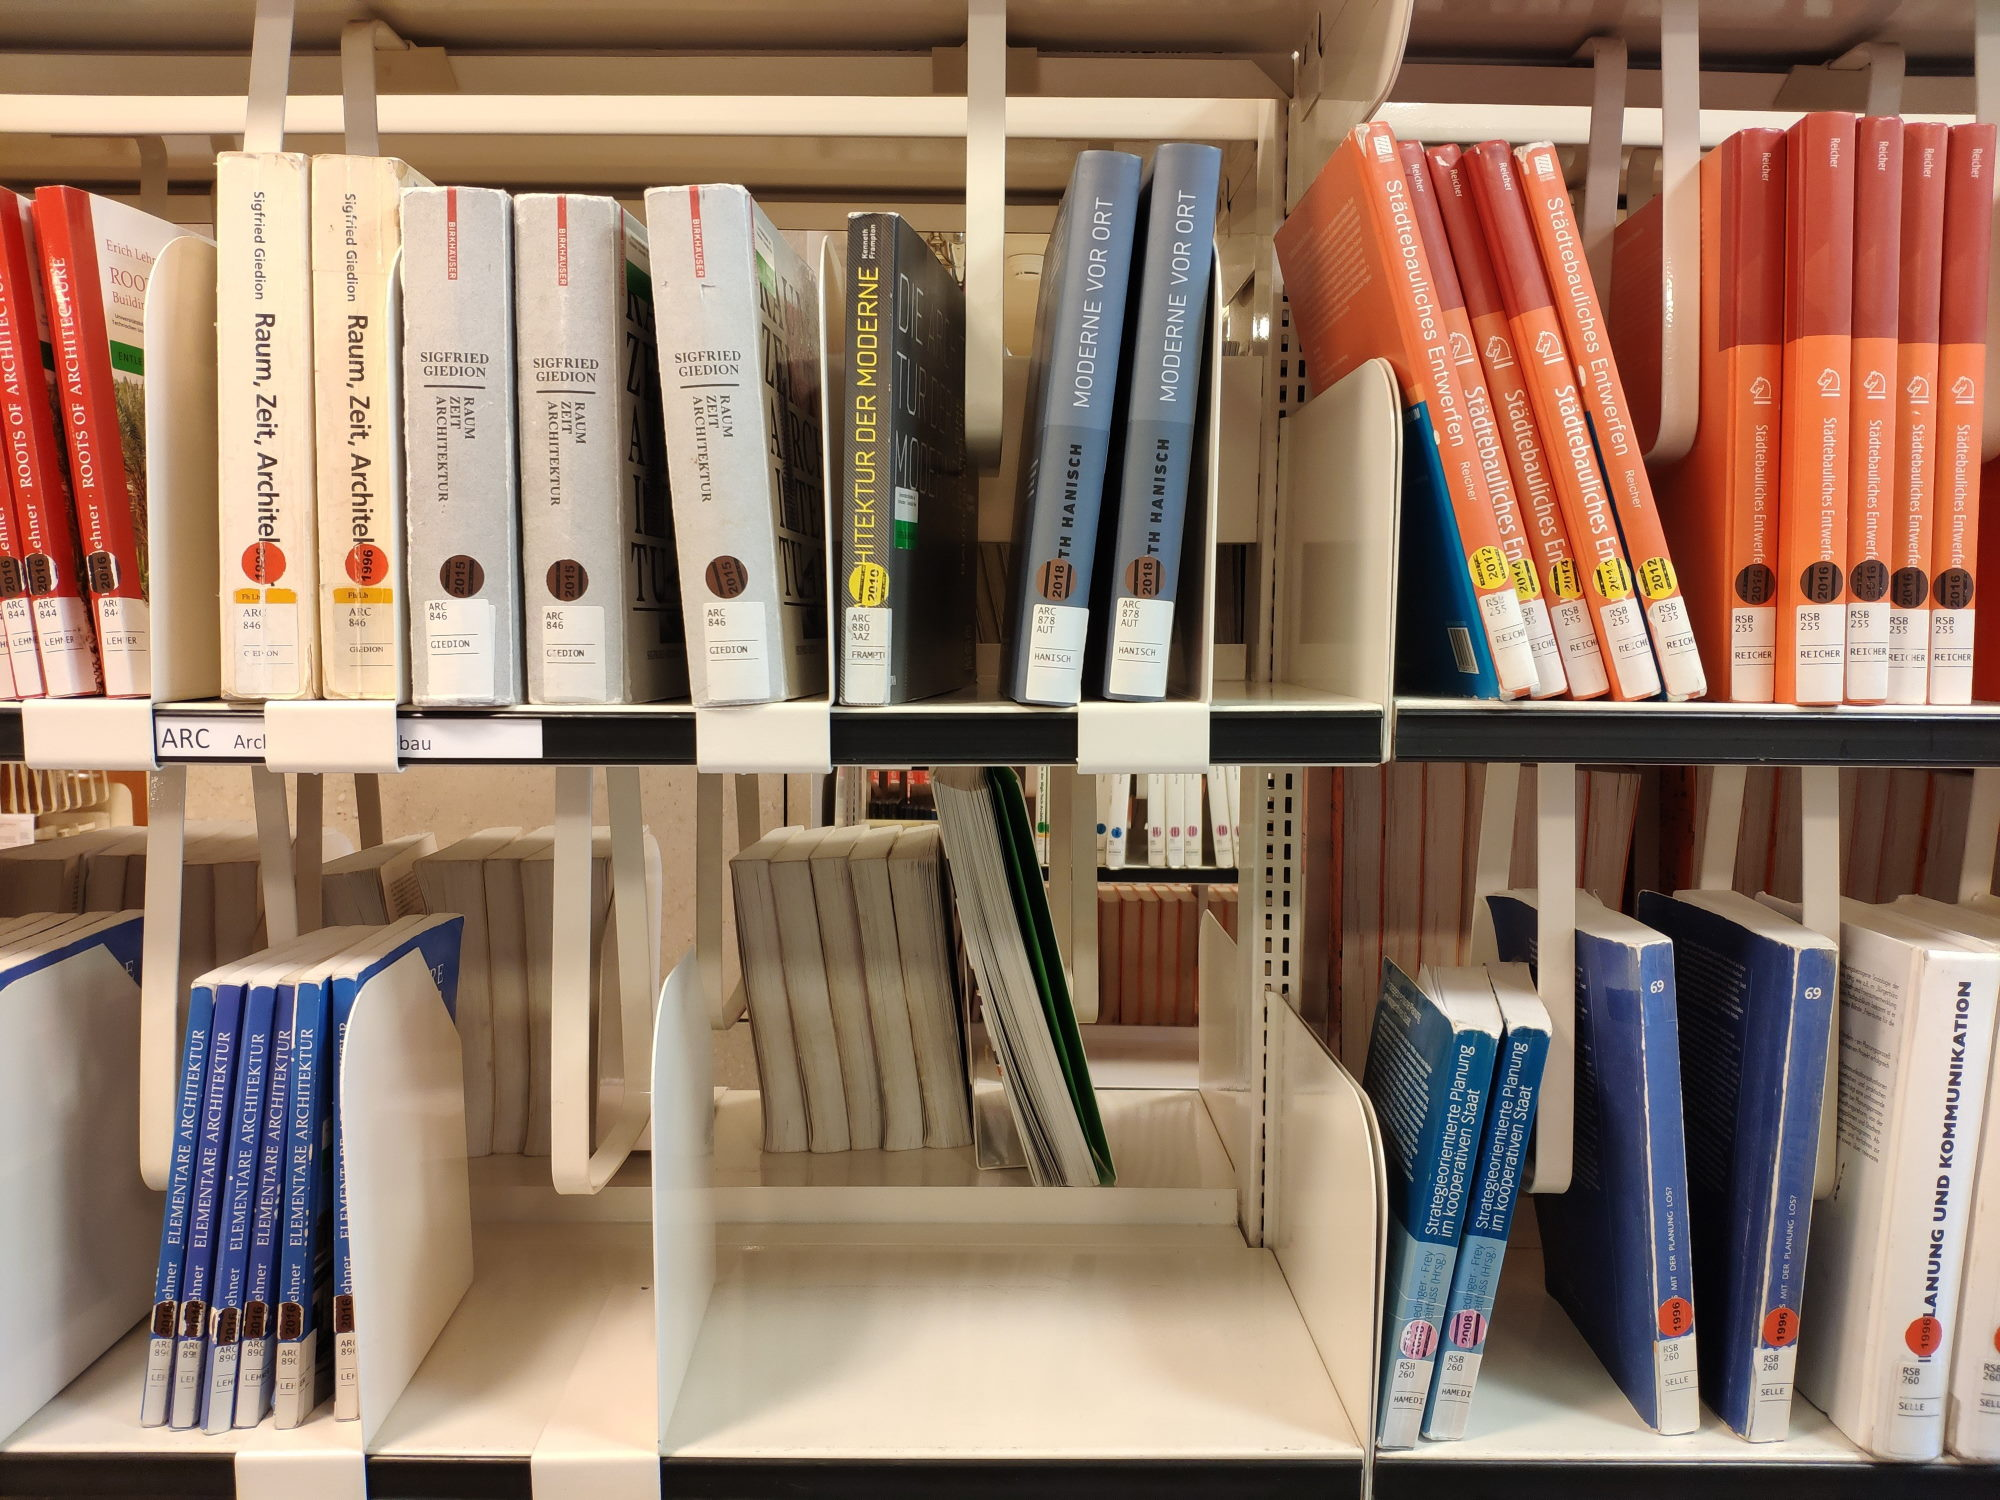
\includegraphics[width=0.4\textwidth]{input.jpg}
 \caption{Input-Bild}
 \label{fig:img}
\end{figure}


\noindent textuell:\\
Strukturierte Klartext-Datei mit Inhalt:
\begin{itemize}
  \item Standort der Bücher (in Büchern zum Ursprung - links-oben)
  \item Vier Pixel-Vektoren, die ein Buch in einem Viereck umschließen
\end{itemize}

\section{Voraussetzungen und Bedingungen}

\begin{itemize}
  \item Die Bücher müssen gerade (+- 5°) stehen.
  \item Das Bild darf nicht mehr als 30° von der Waagrechte abweichen.
  \item Das Bild muss eine für die Texterkennung der Labels ausreichende Auflösung aufweisen (Abhängig von der Entfernung).
  \item Das Bild muss farbig sein.
  \item Das Bild muss ausreichend hell sein. 
  \item Ein Weißabgleich muss durchgeführt worden sein.
\end{itemize}

\section{Methodik}
Methodik- Pipeline
\begin{enumerate}
	\item Hough-Transformation\\
		\textit{Finden der Regalfächer zum Korrigieren der Perspektive}
	\item Persprektivenkorrektur\\
		\textit{Mittels Transformationsmatrix aus HT berechnet}
	\item Eckenerkennung\\
		\textit{Finden der Ecken von Labels}
	\item Integral imaging\\
		\textit{Finden von Labels innerhalb eines Akzeptanzbereichs, es werden nur Bereiche zwischen verschiedenen, zuvor erkannten, Ecken überprüft}
	\item Eigene Heuristik\\
		\textit{Einordnen von Labels in Buch-Koordinaten}
	\item Optical Character Recognition\\
		\textit{Erkennen von Text auf den Labels in den zuvor erkannten Bereichen}
\end{enumerate}

\section{Evaluierung}
\textbf{Interaktion zwischen den Komponenten:}
\begin{itemize}
	\item \textit{Werden die Regalfächer korrekt erkannt?}\\
		  Voraussetzungen:\tab Seite der Regalfächer, die zur Kamera zeigt, ist schwarz.\\
		  Ergebnis:\tab[2.2cm] An jedem Fach liegt eine Gerade an.
	\item \textit{Wird die Perspektive korrekt angepasst?}\\
		  Voraussetzungen:\tab Korrekte Geraden der Regalfächer.\\
		  Ergebnis:\tab[2.2cm] Bücher und Labels sind im Bild weitestgehend rechteckig.
	\item \textit{Werden alle Labels erkannt?}\\
		  Voraussetzungen:\tab Perspektivenkorrigiertes Bild\\
		  Ergebnis:\tab[2.2cm] Bounding-Boxes der gefundenen Labels
	\item \textit{Sind die Bounding Boxes der gefundenen Labels korrekt? Ist der gesamte Text darin enthalten?}\\
		  Voraussetzungen:\tab Korrekt erkanntes Label oder ein false-positive.\\
		  Ergebnis:\tab[2.2cm] Vier Vektoren, die den gesamten Text umschließen (und nicht mehr). Bei false-positives ist das Ergebnis nicht relevant, jedoch sollte es nicht zu groß sein (z.B. das gesamte Bild überdecken).
	\item \textit{Werden die Labels korrekt in Bücher-Koordinaten umgewandelt?}\\
		  Voraussetzungen:\tab Bounding Boxes der Labels sind korrekt.\\
		  Ergebnis:\tab[2.2cm] Bücher-Koordinatensystem als 2D-Array mit Ursprung links-oben.
	\item \textit{Werden die Labels der TU-Bibliothek korrekt gelesen und in Text umgewandelt?}\\
		  Voraussetzungen:\tab Label Bounding-Boxes wurden korrekt berechnet (enthalten keinen unnötigen Text).\\
		  Ergebnis:\tab[2.2cm] String-Repräsentation des Labels. Erwartete Korrektheit: $>$ 90\% für typische Datensätze.
	\item \textit{Wird die Wahrscheinlichkeit der Label-Korrektheit angemessen berechnet?}\\
		  Voraussetzungen:\tab Korrekt in Text umgewandeltes Label.\\
		  Ergebnis:\tab[2.2cm] Floating-point Wert im Intervall [0, 1]. Alle Labels mit Wahrscheinlichkeit 0 wurden entfernt.
\end{itemize}

\textbf{Qualitative Evaluierungsfragen:}
\begin{itemize}
	\item Welche Muster müssen wir in unseren Daten initial erkennen?
	\item Wie muss das Inputbild umgewandelt werden, um eine möglichst effektive Eckenerkennung zu ermöglichen?
	\item Wie versichern wir, dass unser Bild perspektivisch korrekt transformiert wurde?
	\item Welches Indexing ist sinnvoll, und wie signalisieren wir dem User die Bedeutung unserer Indexe?(Buch-Koordinaten)
	\item Welches Pre-Processing ist notwendig, um eine Texterkennung zu ermöglichen?
\end{itemize}

\textbf{Quantitative Evaluierungsfragen:}
\begin{itemize}
	\item Wieviele Bücher erkennen wir durchschnittlich?
	\item Welche Auflösung ist notwendig, um akzeptable Ergebnisse zu erzielen?
	\item Wie wirkt sich der Winkel, in dem das Foto aufgenommen wurde auf die Verwertbarkeit der Labels aus (Erkennung \& OCR)?
	\item Wie wirkt sich der Grad der Befülltheit des Regals auf die Label-Erkennung aus?
	\item Wie wirken sich die Farben und Kontraste der Bücher auf unseren OCR aus?
\end{itemize}

\section{Datenbeispiel}
\begin{figure}[H]
 \centering
 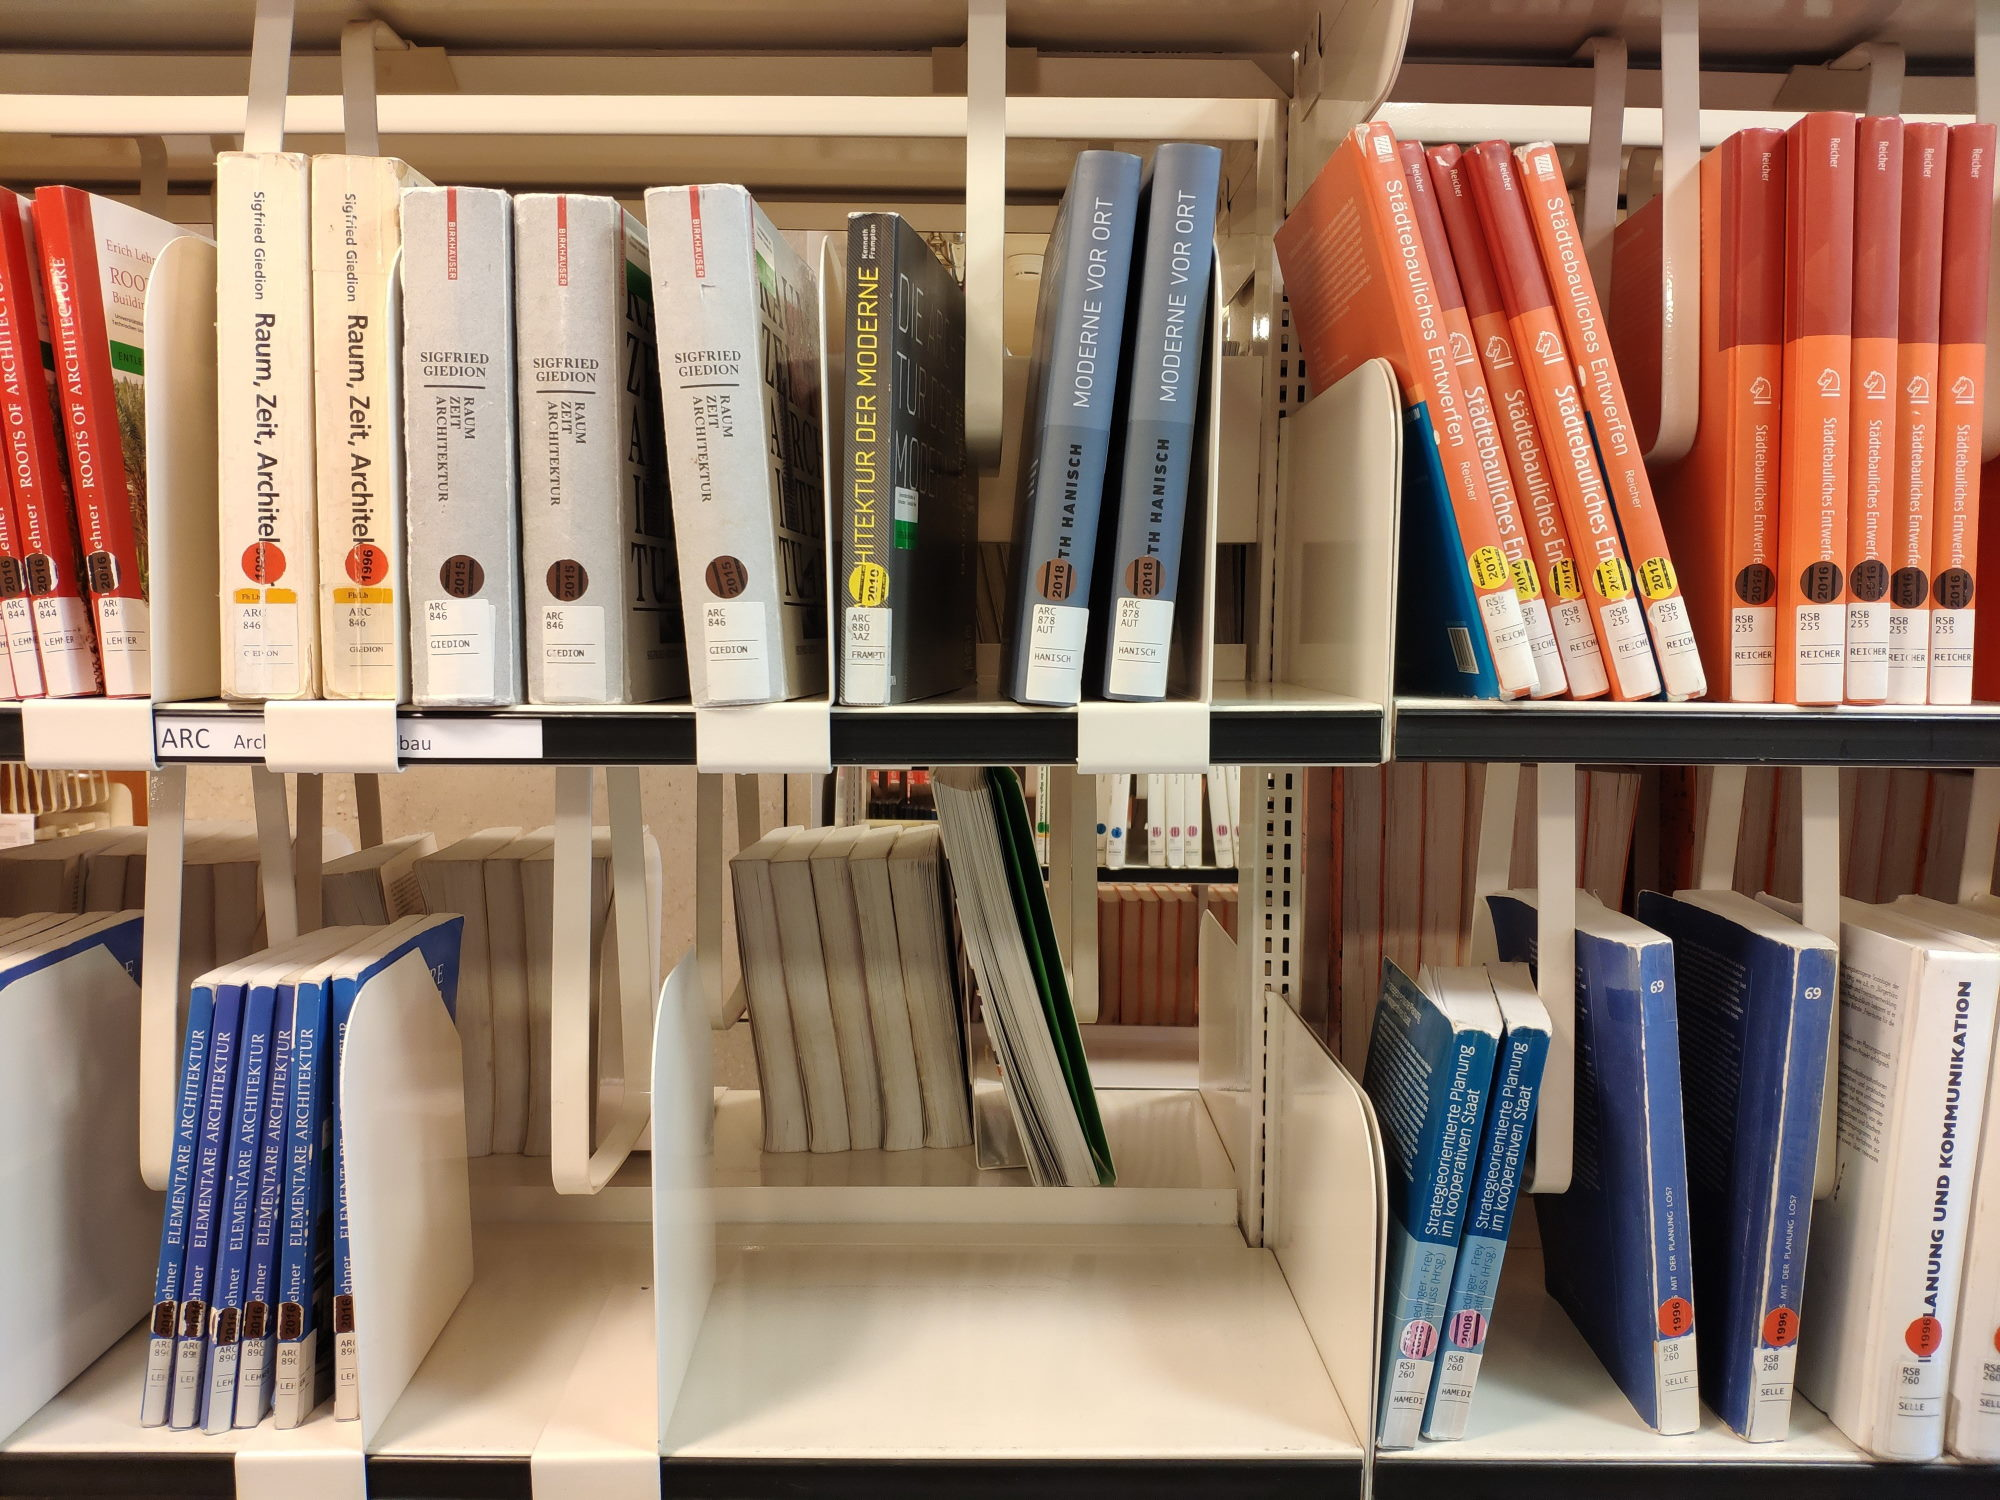
\includegraphics[width=0.4\textwidth]{input.jpg}
 \caption{Input-Bild}
 \label{fig:img}
\end{figure}
\section{Zeitplan}
\begin{table}[h!]
	\centering
		\begin{tabular}{|c|c|c|}
		\hline
		Meilenstein & abgeschlossen am & Arbeitsaufwand in h\\
		\hline
		Prototyp & 10.11. & 30\\
		\hline
		Hough-Transformation & 17.11. & 50\\
		\hline
		Perspektivenkorrektur & 17.11. & 6\\
		\hline
		Labelerkennung & 25.11. & 80\\
		\hline
		Labels in Buch-Koordinaten & 1.12. & 4\\
		\hline
		Optical Character Recognition & 10.12. & 110\\
		\hline
		Labels filtern & 15.12. & 6\\
		\hline
		Daten in Output-Format umwandeln & 15.12. & 4\\
		\hline
		Tests & 18.12. & 5\\
		\hline
		Evaluierung & 20.12. & 5 \\
		\hline
		\end{tabular}
\end{table}

%%------------------------------------------------------
\bibliographystyle{plain}
\nocite{*}
\bibliography{edbv_lit}
%%Bei verwendung von Latex schreibt ihr eure Referenzen in ein eigenes bib-File (siehe hier Beispiel in edbv_lit.bib). Weitere Information zum Einbinden von BibTex gibt es hier: http://www.bibtex.org/Using/de/
%%------------------------------------------------------

\end{document}
